\noindent
\initial{P}lanet Earth is often called the blue planet due to the dominant blue areas visible when viewing Earth from space.
The blue areas are our vast oceans covering more than 70\% \cite{WikiEarth} of the surface.
These oceans contain and support a broad spectrum of life, and are also a great influence on the climate and weather on Earth.
As a matter of fact, all species on Earth are dependent on water in order to survive.
A human can only survive for 5 days without water \cite{SurviveWater}, and even extremophiles called xerophiles, dry loving bacteria, needs a tiny amount of water in order to function.
In other words, water is essential to life as we know it and therefore extremely interesting. 

A single water molecule consists of three atoms, one oxygen atom and two hydrogen atoms.
The two hydrogen atoms are bonded covalently to the oxygen atom.
Due to two lone pairs on the oxygen, meaning electrons that are not shared between atoms, the overall structure of the molecule is bent.
Furthermore, the oxygen atom is much more electronegative than the hydrogens creating a dipole moment in the molecule.
This means that the oxygen will contain a slight, but significant negative charge while the two hydrogens appear as slightly positive.
This creates the basis for the formation of an intricate network of hydrogen bonds as we know that positive and negative charges attracts one another.  

So what makes water so unique?
First of all, the formation of hydrogen bonds gives water a high evaporation entalphy and therefore a large evaporation temperature.
To transform water from its liquid phase to vapor, energy must be applied bringing water to a temperature of 100\degree C.
On the other end of the scale, water will freeze at 0\degree C transforming to ice, which brings us to the second uniqueness of water.
In most cases, a solid phase will be denser than a liquid phase making it sink to the bottom \cite{SolidWater}.
For water this is not the case, as we all have seen polar bears floating on ice flakes in the Arctic.
This phenomenon has had a greater importance than just serving as a fleet for polar bears.
Without this property, ice would have sunk to the bottom in repeated cycles until there was no more liquid water during the cold periods in the history of Earth.
To sum up, due to chemical and physical properties, water remains liquid over a uniquely broad range of temperatures.

However, this only applies when the pressure is 1 atm, or 1 atmosphere, that is the pressure at sea level on Earth.
It seems that pressure and temperature are connected, they both affect the state of all matters.
At the very top of Mount Everest, water boils at 70\degree C \cite{WaterEverest}, making it hard to boil an egg.
The diagram shows how this relationship between temperature and pressure affects the states of water.

\end{multicols}

\begin{center}
	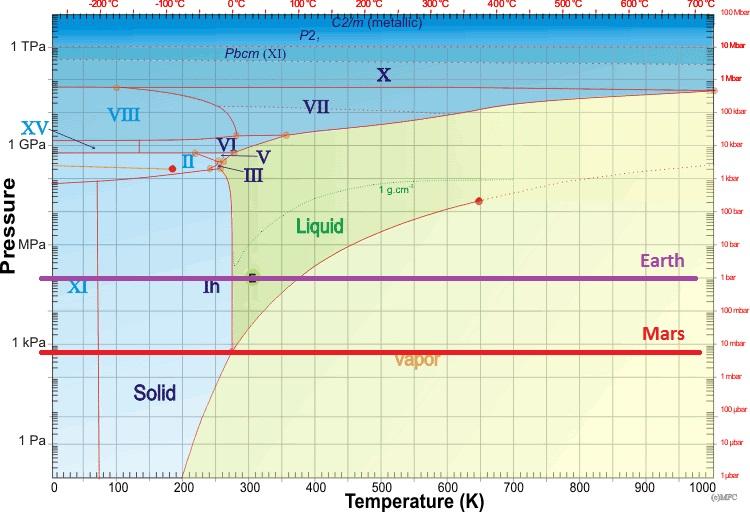
\includegraphics[width=0.9\textwidth]{water_phase_diagram_2_merka.jpg}
	% kilde: http://www1.lsbu.ac.uk/water/water_phase_diagram.html
\end{center}

\begin{multicols}{2}

Notice that although water can appear at Earth's 1 atm, which is about 101 kPa \cite{AtmEarth}, the pressure of 0,6 kPa at the Martian surface \cite{AtmMars} does not allow water to be liquid.
An attempt to melt ice on Mars will result in sublimation.
The mean temperature on Earth is 15\degree C \cite{WikiEarth}, along with the pressure of 1 atm it makes Earth a perfect place for liquid water. 
So far, we have established that we have a lot of water on Earth, and it occurs mostly in its liquid form.
The question remaining is, what is so important with liquid water?

Liquid water has functions as both a solvent and a transport medium.
Both organic and inorganic compounds can be dissolved in water, making it a vital part of the human metabolism.
The blood stream is an essential transport network delivering oxygen and nutrients in our body.
Human blood plasma, the liquid part of the blood, consists of 92\% water \cite{Blood}.
On Earth we have yet to find an organism completely independent of water. 
In fact, in all three theories concerning the origin of life, water was given a leading role as a solution bringing the organic molecules together. 
Since water is vital for living organisms on Earth, it seems appropriate to base our search for life in space on the search for water.
The importance of water is also reflected in NASAs guiding policy: Follow the water \cite{NASAwater}. 
Water is not a rare molecule in space, in fact oxygen and hydrogen are some of the most abundant atoms in the Universe.
The only problem is that the water in space most often is in the solid form of ice, and in rare occasions in form of gas.
There have been discoveries of water on Mars. 
Both poles include ice caps containing solid water and carbon dioxide \cite{MARSwater}. 
Unfortunately, solid water does not have the same solvating and lubricating properties as liquid water, and will therefore not support molecular processes essential for life.
However, dry channels and craters probably formed by erosion suggest that liquid water (or some other liquid) once was present on Mars.
The best signs of life in space is therefore the discoveries of molecules we know can only be formed in contact with water.
For example, in 2002, Mars 2001 Odyssey, which is orbitting Mars, found the spectral signature of hematite, a molecule formed in water. 
This mineral was later discovered by Opportunity, one of the two twin rovers exploring Mars from 2004 to 2010.
Furthermore, in 2005, Spirit, the other twin, found high concentrations of carbonate which originates in wet, near-neutral conditions. 
Carbonate actually dissolves in acid, which means that the water on this area could not be acidic.
The rover roaming the surface of Mars today, named Curiosity, continues seeking for evidence of water. 
Where there is liquid water, there might be alien life. 